\documentclass[a4paper]{article} 

\usepackage[utf8]{inputenc}
\usepackage[T1]{fontenc}
\usepackage{geometry}
\geometry{a4paper}
\usepackage{amsmath}
\usepackage{amsthm}
\usepackage{graphicx}
\usepackage{subcaption}
\usepackage{rotating}
\theoremstyle{plain}
\newtheorem{Lemma}{Lemma}
\newtheorem{Proposition}{Proposition}
\newtheorem{theorem}{Theorem}
\theoremstyle{definition}
\newtheorem{definition}{Definition}
\usepackage{rotating}
\usepackage[english]{babel}
\usepackage{setspace}
\usepackage{copyrightbox}
\usepackage{stackengine}
\usepackage{lscape}
\usepackage{indentfirst}

\begin{document}



\vspace {40mm}

\begin {center}

\vspace {40mm}
\Large

{\bf Covid-19 and the Role of Economic Conditions in \\ French Regional Departments}

\normalsize
\vspace {5mm}

Victor Ginsburgh\\

\small 
ECARES, Universit\'e libre de Bruxelles\\
and CORE, Universit\'e catholique de Louvain

\vspace {5 mm}

\normalsize
Glenn Magerman\\ 

\small 
ECARES, Universit\'e libre de Bruxelles\\
\normalsize
\vspace{5mm}

Ilaria Natali\\

\small 
ECARES, Universit\'e libre de Bruxelles\\
and I3h, Universit\'e libre de Bruxelles
\vspace {10mm}

May 28, 2020
\vspace {5mm}

\end{center}
\normalsize
\begin {abstract}
The recent outbreak of Covid-19 has infected the world at an incredible speed. While there are many similarities across countries in terms of the characteristics of the epidemic spread, there are also large differences across regions. In this paper, we examine regional variation in the outbreak across continental France. We use information on the number of deaths and discharged patients from Covid-19 and socio-economic variables at the department level. Controlling for other factors, we corroborate existing evidence that, unfortunately, inequality kills: departments with more inequality face a higher incidence rate of the disease, expressed as the number of deaths and discharged (gravely ill) patients. Using covariance analysis combining both deaths and releases, we find no statistically differential relationship across factors that contribute to deaths or recoveries.

\vspace{10 mm}
\noindent Keywords: Covid-19, France, departmental effects on the pandemic.\\
JEL codes: I10, I14.

\end{abstract}

\newpage

\section{Introduction}

The outbreak of the Covid-19 pandemic has found both the scientific community and the general public unprepared. Its rapid spread and the skyrocketing number of individuals dying for the virus have caused deep concerns, profound uncertainty and anxiety around the globe. The pandemic not only affects individual health and health care systems, but also economic and sociologic ecosystems. Flattening the curve affects our behavior, but our behavior also affects the curve. In this paper, we aim at understanding how existing socio-economic disparities might contribute to differences in the spread of the virus.

Our concern is to study whether regional variations in socio-economic conditions (poverty level, education level, density of doctors), as well as geographic circumstances (the East and North-east borders with Germany, Luxembourg and Belgium) have an influence on the pattern of the pandemic in continental France.\footnote{We do not include Corsica, la R\'eunion, islands in the Atlantic Ocean, and French Guyana.} Figures 1 and 2 show the 94 French continental departments, and the intensity of the outbreak in these regions. Figure 1 depicts the total number of Covid deaths by department on April 20, 2020. Figure 2 shows the total number of discharged Covid patients on the same day. Clearly, the North (Belgian and Luxembourg borderline) and North-East regions have been hit harder, relative to the South-West areas, as can be explained by the initial hotbeds of Alsace and Bas-Rhin (Low Rhine) regions. France recently decided to pursue confinement in the Eastern regions as well as in Paris and its surrounding  departments, but unlock in the Western and central parts of the country. On May 5, 2020, the President of the Bas-Rhin department in  Alsace claimed that it would be `pure madness' to unlock his department. The French Prime-Minister unveils, at the same time, that France `is cut into two pieces' (Huffpost, 2020). Herv\'e le Bras (2020), researcher at the Institut national d'\'etudes  d\'emographiques, analyzed the dynamics of the pandemic, comparing how the virus developed in two regions: the Haut-Rhin department, where the  number of cases of Covid is large and somewhat out of control, and Bouches-du-Rh\^one in the South,  where the epidemic took off much later. 

In this paper, we use information on socio-economic variables and Covid data to understand how socio-economic variation might contribute to these differences. We implement a simple estimation setup, with lagged socio-economic indicators (year 2017), and current Covid data (April 2020). We do not look at the dynamics, nor at demographic variation at the regional level. We run regressions of both deaths and discharged (D \& D in what follows) separately, as well as together (using an analysis of covariance framework) on a certain number of departmental geographic and  socio-economic characteristics, such as total population, Gini coefficients to measure inequality, level of education, and doctors' density.  

Unfortunately, it was not possible to know with certainty the exact moment at which the epidemic started in each department. Though some figures on cases are available, this information is rather scant before March 18, 2020. In addition, it may have been difficult for public authorities themselves to identify the so-called `patient 0.' This poses, of course, reliability issues for data proceeding March 18. However, we downloaded data on the cumulative number of deaths and patients discharged from hospitals on April 20 when both authorities and the general public were well aware of the pandemic and the collection of data had become more rigorous and well organized. The problem here is that the number of days between `patient 0' and April 20, is not the same in all departments. It is even suggested that a few cases of Covid appeared in France  in December 2019, or even earlier on November 16, 2019, long before blazing, in the department of Haut-Rhin (Peillon, 2020).\footnote{As will be seen, the pandemic was, and still is very serious in the Eastern France.}

It is worth pointing out that Desmet and Wacziarg (2020) have a similar paper, written at about the same time. They concentrate on over 3,000 American counties with an average area of 2,900 sq. Km, while we use information on 94 French departments with an average area of 6,800 sq. km. They consider two outcomes, that is, the cumulated number of cases and deaths at a given date,\footnote {Including those with zero cases and deaths, which we do not do, though there are only two such departments in our data.} while we use the cumulated number of discharged and deaths. They also exploit cross-county variation for their analysis, but they follow the development of epidemics by running regressions day by day. Instead, we exploit cross-department variation by choosing one date, representing one of the \lq high points' of the pandemic. 

They work by using a large set of covariates, while we preferred to focus on a few (neighboring departments with strong attacks of the pandemic, essentially, the North-Eastern border with Belgium, Luxembourg and Germany, and Paris with its surrounding departments; population; inequality measured by the Gini coefficient; level of education and doctor's density).

The two papers are close, in that they use similar approaches and results are comparable, at least for some covariates. An important difference to consider, instead, is that US counties are twice as small as French departments, which may obviously have consequences on driving habits, since one may assume that Americans move more across counties than French people across departments.

The paper is organized as follows. In Section 2, we describe the econometric model and the variables that are used. Section 3 is devoted to econometric results, and  Section 4 concludes. 

\section{The econometric model and data}

We believe that, in this specific context, reverse causality is not an issue, though our results do not identify causal effects since an omitted-variable problem may still exist. The econometric model we use is simple. We regress the number of Covid deaths and discharged from hospitals on departmental variables:
$$y_{ik}= R_i\alpha_k + X_i\beta_k + \epsilon_{ik}, i =1,..., 94; k= 1,2, $$ 

\noindent where $i$ is one of the 94 departments, $y_{ik}$ is either the number of deaths ($k=1$) or of discharged inhabitants ($k=2$) in department $i$, $R_i$ is a vector of two dummy variables which represent geographical characteristics (Northern and Eastern France, and Ile de France, that is Paris and its surroundings), $X_i$ is a vector of departmental socio-economic characteristics, $\alpha_k$ and $\beta_k$ are vectors of parameters and $\epsilon_{ik}$ is the error term. Variables $y_{ik}$ and population, which is one of the variables in vector $X_i$, are expressed in logarithms.

The dependent variables were downloaded  on April 20 from the website  Sant\'e Publique France. The choice we had was to take the more recent data at the time we started our analysis, though they were slightly declining afterwards. We chose the high point of the pandemic.

The vector of two dummy variables $R_i$ includes the following borders: (a) Northern and
Eastern departments that have a border with Southern Belgium, Luxembourg and Germany,\footnote{The following French departments are part of this border: Nord (department number 59), Ardennes (68),
Meuse (55), Meurthe-et-Moselle (54), Bas-Rhin (67), Haut-Rhin (68) and Moselle (57). We excluded a certain number or Eastern departments, that border Switzerland (essentially mountains, though Geneva is quite close to France) as well as the Italian and the Spanish borders, for the same reason (the Alps and the Pyrenees), though Italy and Spain were hardly hit by the virus.} as well as (b) Ile de France, a group of departments, with Paris (75) as center.\footnote{The other departments are Essone (91), Hauts-de-Seine (92), Val-de-Marne (94), Oise (60), Seine-Saint-Denis (93),  Val d'Oise (95), and Yvelines (78).} 

Data for the variables in vector $X_i$ are all downloaded from the INSEE  (Institut National de Statistique et des Etudes Economiques) website and include: number of inhabitants in logs, Gini coefficient, basic education,\footnote{Education levels are census data  available for 1999, 2010 and 2015. Data after 2015 are extrapolated. INSEE provides the number of individuals older than 16 who do no longer attend school (`population non-scolaris\'ee') in each education group. Basic Education, here, is defined as the share of those with no diploma or with a Dipl\^ome National du Brevet (DNB), which is granted after completion of the first cycle of education, or with a Brevet d'etude professionnelle (BEP) or Certificat d'apritude professionelle (CAP), which are obtained after completing the first two years of a professional high school.} number of doctors per 100,000 inhabitants.

We ran five regression for D \& D, by introducing variables one after the other, in the order described above. The first two contain the dummies {\em North-East} and {\em Ile de France}; next comes population,\footnote{We also tried population density in place of population (all combinations), but population performs best.} inequality within regions measured by the Gini coefficient\footnote{Regressions including the GDP per head exhibited no association between the latter and our outcome variables},  education and density of doctors. 

\section{Results}
\subsection{Baseline Regressions}
Results appear in Tables 1 (for deaths) and 2 (for discharged) and are very similar across the two tables. Clearly, the North-Eastern border and Ile de France (column 1) have the largest number of D \& D people. This may be partly due to the fact that departments in the North-East and, especially, in Ile de France, which includes Paris and the surrounding departments, are among the most populated ones. This becomes obvious in column (2), where we add the variable population, which causes a drop in the magnitude of the coefficients for both dummies (and a larger drop for the dummy \textit{Ile de France}). Despite this, coefficients picked up by the two dummies remain significantly different from 0 at the 0.01 probability level. Population only can thus not fully capture the extension of the virus in these two regions.

Next, we add the Gini coefficient. In both regressions the variable picks up positive effects that are all significantly different from 0, at the 0.01 or 0.05 probability level. This means that a larger level of inequality is associated with a larger number of deaths and severely ill individuals. This is an important result and seems to be in line with previous findings in the UK. According to an article published on \textit{The Guardian}, poorer areas in England and Wales are significantly more affected by the pandemic, with twice a death toll as more affluent neighborhoods. This may be due to a few reasons: for instance, individuals in a disadvantaged economic status are more likely to have pre-existing conditions, they are more likely to live in worse quality housing, they are more likely to have jobs that cannot be done through smart-working (by staying at home). These are, evidently, factors that contribute to expose more the most vulnerable populations to the virus.    

The effect of poor education, as described earlier, is probably overshadowed by the effect of inequality, that is, large differentials in incomes within each department. People without higher education are likely to remain poor. The coefficients picked up by the variable are  not significantly different from 0.

Finally, we get to those who have been of great help in the corona pandemic. One expects that more physicians per inhabitant would help containing the outbreak, by allowing people to enter a hospital quickly enough and by providing them with the necessary treatment. Indeed, here, the density of doctors (both generalists and specialists) is negatively associated to both the number of deaths and the number of individuals severely affected by the virus, as proxied by the number of discharged. The coefficients are, however, not statistically different from zero, which may be due to the presence of some other (confounding) factors that we are not taking into account. 

\subsection{Analysis of Covariance}
The estimated parameters displayed in Tables 1 and 2 do not seem to be very different, though Table 1 deals with death, while Table 2 deals with those who were discharged from hospitals. To check whether they are significantly different, we opted using an analysis of covariance, which implicitly assumes that the distribution of errors is the same in both subsamples (D \& D). The model is now:
$$y_{i0}= R_0 \alpha_0 + X_0\beta_0  +  \delta R_0\alpha +  \delta X_0\beta + \epsilon_{i0}, i =1,..., 186.$$

\noindent In this formulation,  $y_{i0}$ is a vector constructed by piling up each department's deaths followed by each department's discharged and is regressed on a matrix $R_0$ formed by piling up two matrices $R_i$. Matrix $X_0$ is constructed in the same way by repeating twice $X_i$. Finally, $\delta$ is a dummy variable equal to 1 for observations related to $y_{i1}$, that is, deaths, and 0 for discharged. The coefficients on the interaction terms $\delta R_{0}$ and $\delta X_{0}$ will tell us whether the effect of the covariates is different for deaths and discharged.\footnote{Note that the number of observations should be equal to $2\times 94$, since there are 94 departments, but two observations on the variable $y_{i1}$ are missing (see above).} The results that we now analyze can be found in Table 3.

As can be checked, the coefficients picked up by the variables North-East, Ile de France, Population, Gini,  Education and Doctors' density, as well as the value of the intercept, are exactly the same as those in Table 2. This is due to the fact that our dummy, $\delta$, is equal to zero for discharged and, hence, these coefficients pick the effect of the covariates on the number of discharged individuals. Those coefficients that were significantly different from 0 remain so, and those that were not, remain so as well. Standard errors are also approximately the same. 

The estimates for $\alpha$ and $\beta$, instead, will tell us the difference in the effect of each independent variable across the two groups (deaths and discharged). To make this clearer, consider the following example: in Equation (5), results show that the effect of North-Eastern regions is equal to 0.955 for the group of discharged (as in Table 2), to which 0.242, picked up by the interaction $\delta R_0$, should be added for those who died. The sum is equal to 1.197 and it is identical to the coefficient associated to North-East in column 5 of Table 1. This shows that the coefficient associated to each interaction term will yield the difference in the effect of each covariate across the two groups: if this coefficient is not statistically different from zero, we conclude that this difference is not significant.

The estimates of $\alpha$ (associated to the interactions North-East*Dummy and Ile de France*Dummy) are positive and significantly different from  0 at the 0.01 or 0.05 level, which implies that they increase the role of the two regions for those who have died, in all regressions. 

The effect of Population is common across the two groups (D \& D) since the coefficient for Dummy*Population is not significantly different from 0. Analogous reasoning applies to the Gini since the Dummy*Gini coefficients are not different from zero. Finally, Education and Doctors' density  do not contribute to the fits. It is also interesting to note that the coefficient for Dummy*Intercept is negative (but small and not significantly different from 0 in Equations (2) and (3)) which indicates that the number of deaths is (fortunately) smaller that the number of discharged, on average. 

It is also worth noting that all fits of equations (3) to (5) are good since the adjusted $R^2$ are larger than 0.65 and increase to 0.73 in the analysis of covariance in Table 3.



 %$$
%\left \{  
%\begin {tabular} {ll}
% $y_{i1}$\\
% $y_{i2}$
% \end {tabular}
% \right \}
% = R_i\alpha_0 + X_i\beta_0 + \delta R_i \chi+ \delta X_i\psi + \epsilon_{i0}, i =1,..., 186.
%$$
 
 %Observations $y_{i1}$ = for deaths and $y_{i2}$ for recoveries are piled up one after the other as one vector $y_{i0}$, which is regressed on $R_{i0}$ the matrix of the two regional variables and , also repeated  twice 

\section {Conclusions}  

There is a clear pattern of heavy infections (deaths and discharged patients) along the French border with Belgium, Luxembourg and Germany, and in the departments that surround  Paris. It is not clear whether the effect of the border is due to the countries that border France (and people passing from one country to the other), or to a cause that we did not find. This is different for Ile de France with over 12 million inhabitants, who, before confinement, were traveling, usually using metros or trains in and out of Paris, where they work (or vice-versa). Note that more recently, that is, after inputting the numbers of D \& D, the virus moved to more central and western regions,\footnote{Auvergne, C\^ote-d'Armor, Franche-Comt\'e, Loiret, Pays de Loire, Vend\'ee,  and other regions. See Direct Coronavirus en France : bilan, nouveaux cas et foyers https://www.topsante.com/medecine/maladies-infectieuses/zoonoses/coronavirus-en-direct-nouveaux-cas-foyers-en-france-634781 [last consulted on May 19, 2020].} though with less virulence than in the North-East and Ile de France. We will need, however, to wait a couple of weeks, to check whether this will remain milder.

The fact that population is related to D \& D is obvious, but far from being the only factor, as we showed above.

Finally, it should be clear that more inequality means that the population is not homogeneous, and that richer people live in one part of a town or a village, are probably more careful, and may have gardens to be able to breath, while poor people have little choice, live in another part of the town and are more likely to walk on the street and in parks.  This is what a British report also points out (Improvement Service, 2020, p. 3):

\begin{quote}
"People living in socio-economic disadvantage are more likely to be working in the
low paying jobs which are keeping the country going in supermarkets, as cleaners,
delivery drivers and home care workers, and a significant proportion of these low
paid workers will be women. The four `C's' of cleaning, care, cashiering and catering,
commonly seen as women's work are now massively important, and those working
in these areas are being exposed daily to the risk of contracting Covid-19."
\end{quote}

They are also more likely to have lost (at least for some time) their job, which is a very grim perspective.

As we said, the estimated coefficients picked up by education, which are not significantly different 0, are probably in the shadow of unequal incomes measured by the Gini coefficient. The fraction of poor people who usually have a low level of education  are less likely to escape the pandemic.

Most crises are likely to increase inequality, given increases in the rate of unemployment and lower wages that follow, as well as difficulties to get loans from banks to pay their mortgage, even if they are only temporary. And Covid-19 will probably not be different. 
This means that the pandemic hits harder areas in socio-economic disadvantage today and will probably exacerbate disparities in the near future (Furceri et al., 2020). This highlights the importance of policy interventions aimed at helping individuals living in poor conditions, in order to (i) attenuate the impact of the pandemic today and (ii) attenuate the (potential) negative consequences of the pandemic in the near future. \\


\newpage
\section{References}

\begin {description}

\item Desmet, Klaus and Romain Wacziarg (2020), Understanding spatial variation in Covid-19 across the United States, NBER Working Paper 27329.

\item Furceri, D., Loungani, P. L., Ostry, J. D. and Pizzuto, P. (2020). COVID-19 will raise inequality if past pandemics are a guide.  {\em VOX CEPR Policy Portal} [web: last accessed May 20, 2020].

\item Le Bras, Herv\'e (2020). On entrevoit trois stades de l'\'epid\'emie de Covid-19 en France. {\em Le Monde}, April 30, 2020.

\item Huffpost (2020). D\'econfiner les d\'epartements rouges? De la `pure folie' pour le pr\'esident du Bas-Rhin, {\em Le HuffPost}, May 8, 2020

\item Improvement Service (2020), Poverty, inequality and Covid-19  [web: last accessed May 20, 2020].

\item Peillon, Luc (2020). L'origine de l'\'epid\'emie de Covid en France peut-elle remonter \`a l'automne 2019? {\em Lib\'eration}, 21 mai 2020.

\item Pidd, H., Barr, C. and Mohdin, A. (2020). Calls for health funding to be prioritised as poor bear brunt of COVID-19.  {\em The Guardian}, May 1, 2020.

\end{description}

\newpage
 \begin{figure}[htbp]
%\caption*{Figure 1. Parallel Trend Assumption: Treatment vs Control Group\label{fab1}}
\centering
\def\stackalignment{l}
\fbox{\stackunder{\includegraphics[scale=0.80]{Map_Deaths.eps}}
{Sources: Santé Publique France; authors' calculations.}}
\end{figure} 

 \begin{figure}[htbp]
%\caption*{Figure 2. Parallel Trend Assumption: Treatment vs Control Group\label{fab1}}
\centering
\def\stackalignment{l}
\fbox{\stackunder{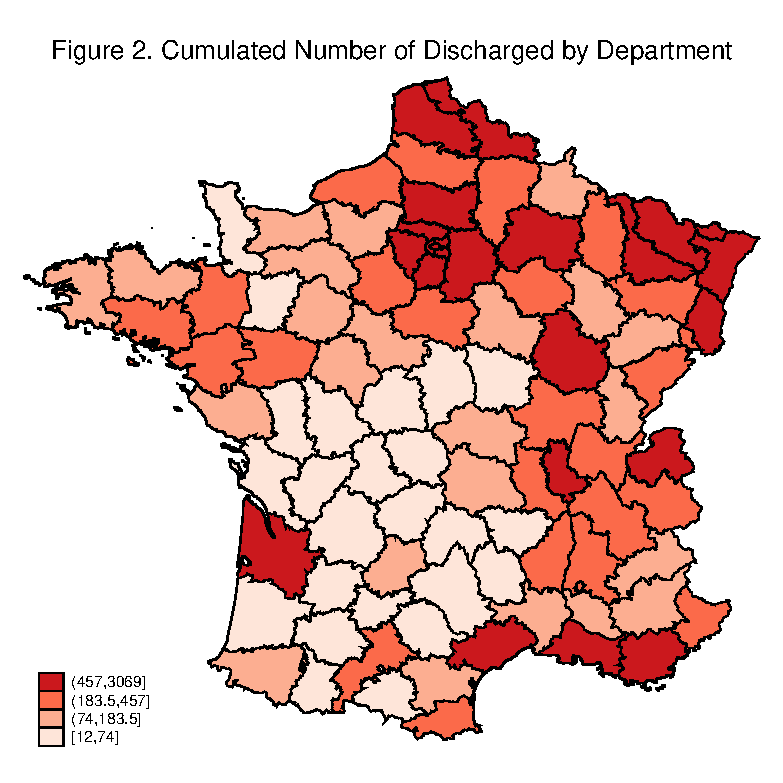
\includegraphics[scale=0.80]{Map_Discharged.eps}}
{Sources: Santé Publique France; authors' calculations.}}
\end{figure} 


\begin{table}[htbp]\centering
\def\sym#1{\ifmmode^{#1}\else\(^{#1}\)\fi}
\caption*{Table 1. Regression Results. Number of Deaths. \label{tab1}}
\begin{tabular}{l*{5}{c}}
\hline\hline
\\
                &\multicolumn{1}{c}{(1)}&\multicolumn{1}{c}{(2)}&\multicolumn{1}{c}{(3)}&\multicolumn{1}{c}{(4)}&\multicolumn{1}{c}{(5)}\\
                &\multicolumn{1}{c}{}&\multicolumn{1}{c}{}&\multicolumn{1}{c}{}&\multicolumn{1}{c}{}&\multicolumn{1}{c}{}\\
\hline
\\
North-East            &     1.78493***&    1.362145***&    1.320606***&    1.199691***&    1.196585***\\
                &  (.4041796)   &  (.2496312)   &  (.2371874)   &  (.2474712)   &  (.2473837)   \\
                \\
Ile de France           &    2.658232***&    1.434573***&    1.212202***&    1.402966***&    1.301863***\\
                &  (.2022909)   &  (.1942773)   &  (.1892048)   &  (.2181983)   &  (.3032876)   \\
                \\
Population  &               &    1.063447***&    .9891452***&    1.158865***&    1.150728***\\
                &               &  (.1446876)   &  (.1619487)   &   (.225545)   &   (.230567)   \\
                \\
Gini            &               &               &    .0538155** &    .0981521***&    .1110501***\\
                &               &               &  (.0268751)   &  (.0295869)   &  (.0363411)   \\
                \\
Education            &               &               &               &    .0470603   &    .0407087   \\
                &               &               &               &  (.0304477)   &  (.0351186)   \\
                \\
Doctors' Density &               &               &               &               &    -.000752   \\
                &               &               &               &               &  (.0011276)   \\
                \\
Intercept   &    3.670147***&   -10.23082***&   -10.65228***&   -16.09139***&   -15.81489***\\
                &  (.1283489)   &  (1.931404)   &  (1.852999)   &  (4.318988)   &  (4.498292)   \\
\\
\hline 
$R^2$              &    .3922114   &    .6461379   &     .652798   &     .665427   &    .6662798   \\
Adjusted $R^2$     &    .3785533   &    .6340744   &    .6368347   &    .6459751   &    .6427231   \\
N               &          92   &          92   &          92   &          92   &          92   \\
\hline\hline 
\multicolumn{6}{l}{\small\textit{Note:} Two of the 94 departments had no deaths on the 20th of April.}    \\
\multicolumn{6}{l}{\small Robust standard errors in parenthesis. $^{*} p<0.1$, $^{**} p < 0.05$, $^{***} p < 0.01$} 
\end{tabular}   
\end{table}









\begin{table}[htbp]\centering
\def\sym#1{\ifmmode^{#1}\else\(^{#1}\)\fi}
\caption*{Table 2. Regression Results. Number of Discharged.\label{tab1}}
\begin{tabular}{l*{5}{c}}
\hline\hline
\\
                &\multicolumn{1}{c}{(1)}&\multicolumn{1}{c}{(2)}&\multicolumn{1}{c}{(3)}&\multicolumn{1}{c}{(4)}&\multicolumn{1}{c}{(5)}\\
                &\multicolumn{1}{c}{}&\multicolumn{1}{c}{}&\multicolumn{1}{c}{}&\multicolumn{1}{c}{}&\multicolumn{1}{c}{}\\
\hline
\\
North-East            &    1.498502***&    1.013639***&    .9433316***&    .9574594***&     .954981***\\
                &  (.3883368)   &  (.2502798)   &  (.2346669)   &  (.2418449)   &  (.2415764)   \\
                \\
Ile de France           &    2.423485***&    1.100784***&    .7230497***&    .6993664***&    .6430911** \\
                &  (.1784774)   &   (.159507)   &  (.1747128)   &  (.2000135)   &   (.264656)   \\
                \\
Population  &               &    1.112531***&     .993284***&    .9752686***&    .9719336***\\
                &               &  (.1123722)   &  (.1211013)   &  (.1553269)   &  (.1580135)   \\
                \\
Gini            &               &               &    .0902798***&    .0848994** &    .0923457** \\
                &               &               &  (.0292446)   &  (.0330915)   &  (.0361311)   \\
                \\
Education            &               &               &               &   -.0055659   &   -.0089142   \\
                &               &               &               &  (.0224333)   &   (.025325)   \\
                \\
Doctors' Density &               &               &               &               &   -.0004245   \\
                &               &               &               &               &   (.001146)   \\
                \\
Intercept          &    4.907909***&   -9.592106***&   -10.37125***&   -9.751786***&   -9.626842***\\
                &  (.1208542)   &  (1.489271)   &  (1.389197)   &  (3.047651)   &  (3.148192)   \\
\\
\hline 
$R^2$               &    .3571441   &    .7118813   &     .733274   &    .7334894   &    .7338071   \\
Adjusted $R^2$     &    .3430154   &    .7022774   &    .7212863   &    .7183468   &     .715449   \\
N               &          94   &          94   &          94   &          94   &          94   \\
\hline\hline 
\multicolumn{6}{l}{\small Robust standard errors in parenthesis. $^{*} p<0.1$, $^{**} p < 0.05$, $^{***} p < 0.01$} 
\end{tabular}   
\end{table}



\begin{table}\centering
\def\sym#1{\ifmmode^{#1}\else\(^{#1}\)\fi}
\caption*{Table 3. Results of the Analysis of Covariance.\label{tab1}}
\scalebox{0.94}{
\begin{tabular}{l*{6}{c}}
\hline\hline
\\
                &\multicolumn{1}{c}{(1)}&\multicolumn{1}{c}{(2)}&\multicolumn{1}{c}{(3)}&\multicolumn{1}{c}{(4)}&\multicolumn{1}{c}{(5)}\\
                &\multicolumn{1}{c}{}&\multicolumn{1}{c}{}&\multicolumn{1}{c}{}&\multicolumn{1}{c}{}&\multicolumn{1}{c}{}\\               
\hline
\\
North-East          &    1.498502***&    1.013639***&    .9433315***&    .9574594***&     .954981***\\
                &  (.3894372)   &  (.2510045)   &  (.2353612)   &  (.2425761)   &  (.2423228)   \\
 \\
North-East*Dummy  &    .2864277***&    .3485058***&    .3772743***&    .2422315** &    .2416038** \\
                &  (.0957056)   &  (.0861668)   &  (.0952936)   &  (.0939364)   &  (.0957339)   \\
 \\
Ile de France         &    2.423485***&    1.100784***&    .7230497***&    .6993664***&    .6430911** \\
                &  (.1789831)   &  (.1599689)   &  (.1752297)   &  (.2006182)   &  (.2654737)   \\
 \\
Ile de France*Dummy &    .2347463** &    .3337892***&    .4891525***&    .7035998***&     .658772***\\
                &  (.0927611)   &  (.1135917)   &  (.1457478)   &  (.1643193)   &  (.2096761)   \\
                \\
Population  &               &    1.112531***&     .993284***&    .9752686***&    .9719336***\\
                &               &  (.1126976)   &  (.1214596)   &  (.1557965)   &  (.1585017)   \\
 \\
Population*Dummy &               &   -.0490841   &   -.0041388   &    .1835962   &     .178794   \\
                &               &  (.1035451)   &  (.1141379)   &  (.1461286)   &  (.1472504)   \\
                \\
Gini            &               &               &    .0902798***&    .0848994** &    .0923457** \\
                &               &               &  (.0293312)   &  (.0331916)   &  (.0362427)   \\
  \\
Gini*Dummy  &               &               &   -.0364643   &    .0132527   &    .0187044   \\
                &               &               &  (.0223767)   &  (.0248453)   &  (.0257238)   \\
                \\
Education            &               &               &               &   -.0055659   &   -.0089142   \\
                &               &               &               &  (.0225011)   &  (.0254033)   \\
  \\
Education*Dummy  &               &               &               &    .0526262***&     .049623** \\
                &               &               &               &  (.0189861)   &  (.0210125)   \\
                \\
Doctors' Density &               &               &               &               &   -.0004245   \\
                &               &               &               &               &  (.0011496)   \\
 \\
Doctors' Density*Dummy &               &               &               &               &   -.0003275   \\
                &               &               &               &               &  (.0008917)   \\
                \\
Intercept          &    4.907909***&   -9.592106***&   -10.37125***&   -9.751787***&   -9.626843***\\
                &  (.1211966)   &  (1.493583)   &  (1.393307)   &  (3.056866)   &  (3.157919)   \\
\\
Dummy*Intercept         &   -1.237761***&   -.6387168   &   -.2810338   &   -6.339603** &   -6.188046** \\
                &  (.0738208)   &  (1.390247)   &  (1.372104)   &   (2.82479)   &  (2.888944)   \\
  \\
\hline 
$R^2$            &    .4825624   &    .7321625   &    .7433982   &     .749052   &    .7495514   \\
Adjusted $R^2$     &    .4681891   &    .7216296   &    .7302765   &    .7331875   &    .7306222   \\
N               &         186   &         186   &         186   &         186   &         186   \\
\hline\hline 
\multicolumn{6}{l}{\small\textit{Note:} Two of the 94 departments had no deaths on the 20th of April. This results into 2*94-2 observations.}    \\
\multicolumn{6}{l}{\small Robust standard errors in parenthesis. $^{*} p<0.1$, $^{**} p < 0.05$, $^{***} p < 0.01$} 
\end{tabular}   }
\end{table}




\end{document}